In the proposed model, planar quadrilateral elements adopting bilinear isoparametric representation of element geometry and shape functions \cite{bathe1976numerical} are coupled with the layered-section model proposed by \cite{lu2015shear}.

A plane-stress concrete material model which was developed based on the three-dimensional model proposed by \cite{faria1998strain}. The formulation is based on continuum damage mechanics and defines a relation between the response in a non-damaged effective space and a damaged physical space through an increasing damage variable. In addition to parameters based on material properties (such as Young modulus, Poisson ration, yield strength, etc.), representation of the material in-plane constitutive behavior is obtained through other four independent parameters: a coefficient $\beta$  governing the plastic strain rate and three damage parameters governing the damage evolution: Ap, An, Bn.



\begin{figure}[!htbp]
  \centering {
    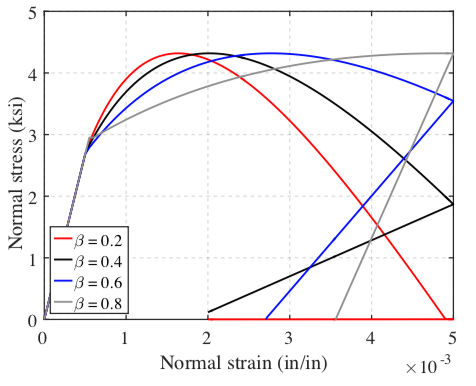
\includegraphics[width=0.7\textwidth]
    {figures/SWIM_beta.png} }
  \caption{ Effect of $\beta$ on the stress-strain relation and damage evolution}
  \label{fig:beta}
\end{figure}

An appropriate selection of the parameters that define the cyclic behavior of concrete is fundamental to capturing the response of RC shear walls at both the global and local level.

Plastic strain rate coefficient, $\beta$ governs the post-yield hardening modulus in the effective (undamaged) space and the plastic strain rate. 
\Cref{fig:beta} shows sample stress-strain relation with complete load removal at strain value of $5x10^{-3}$ to illustrate the effect of $\beta$. 
A higher value of $\beta$ increases the amount of plastic strain accumulated. 
A special case of $\beta$ = 0 represents elastic behavior with elastic unloading. 
Typical values of $\beta$ are 0.3 - 0.6.


\begin{figure}[!htbp]
  \centering {
    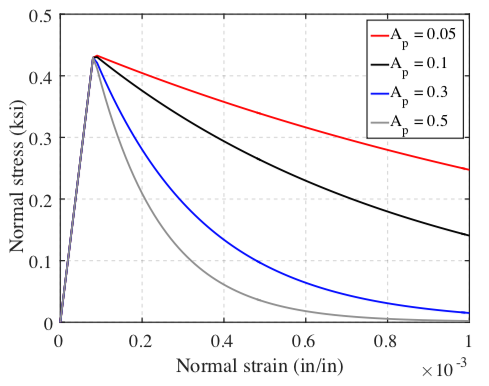
\includegraphics[width=0.7\textwidth]
    {figures/SWIM_Ap.png} }
  \caption{ Effect of Ap on the stress-strain relation}
  \label{fig:Ap}
\end{figure}

Parameter Ap governs the tensile fracture energy and affects the ”ductility” of the tensile response. Fig. 2 shows the effect of parameter Ap on the response in uniaxial tension for different values of Ap. A higher Ap results in a more ductile tensile response. \cite{faria1998strain} suggests an expression to relate Ap to the characteristic length $l_{ch}$ and fracture energy $G_f$:

\begin{equation}
A_p=\left(\frac{G_fE}{l_{ch}(f_t)^2}-\frac{1}{2}\right)^{-1}\geq 0
\end{equation}




\begin{figure}[!htbp]
  \centering {
    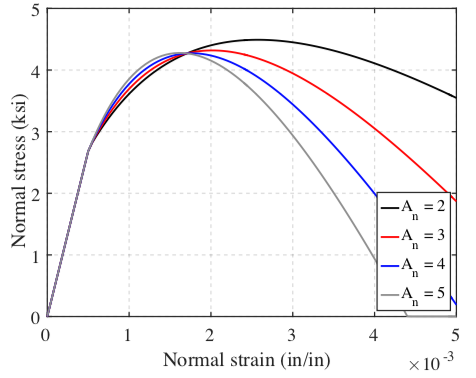
\includegraphics[width=0.7\textwidth]
    {figures/SWIM_An.png} }
  \caption{ Effect of An on the stress-strain relation}
  \label{fig:An}
\end{figure}

\begin{figure}[!htbp]
  \centering {
    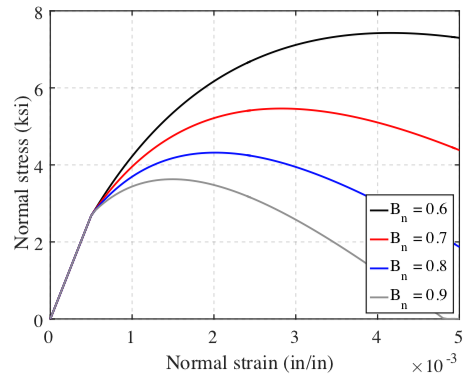
\includegraphics[width=0.7\textwidth]
    {figures/SWIM_Bn.png} }
  \caption{ Effect of Bn on the stress-strain relation}
  \label{fig:Bn}
\end{figure}

Parameters An and Bn govern the softening behavior of concrete in compression. \Cref{fig:An} and \Cref{fig:Bn} show the effect of parameters An and Bn on the response of uniaxial compression for different values of the parameters. 
Both parameters affect the ductility of the compressive response; 
however, parameter An changes the ductility but does not alter the peak strength significantly, 
whereas parameter Bn changes both the ductility and the peak strength. 
It is noteworthy that the numerical solution is rather sensitive to change in parameter Bn.



For modeling reinforcing steel, any uniaxial steel material constitutive model can be used provided it is embedded in the plane stress material object, whereby the steel is assigned a direction and a plane stress tensor is constructed.





